\documentclass[11pt]{article}
\usepackage[utf8]{inputenc}
\usepackage[margin=1.25in]{geometry}
\usepackage{amsmath, amsfonts, amssymb}
\usepackage[dvipsnames]{xcolor}
\definecolor{niceblue}{HTML}{236899}
\usepackage{hyperref}
\hypersetup{
    colorlinks=true,
    linkcolor=niceblue,
    filecolor=black,
    urlcolor=niceblue,
    citecolor=niceblue,
    linkbordercolor = white
}
\usepackage{graphicx}
\usepackage{longtable}
\usepackage{underscore}
% \usepackage{array}
% \usepackage{amsbsy}
% \usepackage{epsfig}
\usepackage{bm}
% \usepackage{xspace}
\usepackage{color}
\usepackage{lineno}
\usepackage{ragged2e}
%$ \usepackage{comment}
% \usepackage{multirow}
% \usepackage{titling}

% Linux Libertine:
\usepackage{textcomp}
\usepackage[sb]{libertine}
\usepackage[varqu,varl]{inconsolata}% sans serif typewriter
\usepackage[libertine,bigdelims,vvarbb]{newtxmath} % bb from STIX
\usepackage[cal=boondoxo]{mathalfa} % mathcal
\useosf % osf for texb, not math
% \usepackage[supstfm=libertinesups,%
%   supscaled=1.2,%
%   raised=-.13em]{superiors}
\usepackage{setspace}

\widowpenalty10000
\clubpenalty10000

\definecolor{darkgrey}{HTML}{A9A9A9}
\renewcommand\linenumberfont{\normalfont\bfseries\small\color{darkgrey}}
\modulolinenumbers[2]

\usepackage{booktabs}
\usepackage[round]{natbib}
\bibliographystyle{mee}
\bibpunct{(}{)}{,}{a}{}{,}
\usepackage{authblk}
\usepackage{pdflscape}
\usepackage{setspace}

\date{}

\title{Approximating spatial processes with too many knots degrades predictive accuracy of SPDE models}

\author[1]{Eric J. Ward}
\author[2]{Sean C. Anderson}

\affil[1]{Conservation Biology Division, Northwest Fisheries Science Center, National Marine Fisheries Service, National Oceanic and Atmospheric Administration, 2725 Montlake Blvd E, Seattle WA, 98112, USA}
\affil[2]{Pacific Biological Station, Fisheries and Oceans Canada, Nanaimo, BC, V6T 6N7, Canada}
\affil[*]{corresponding author: eric.ward@noaa.gov}

\linenumbers
% \doublespacing
% \onehalfspacing
\singlespacing

\begin{document}

\maketitle

\abstract{
\begin{enumerate}
\item
  Spatial and spatiotemporal models are increasingly used in ecology.
  Applications have used these methods to track population change over
  time, assess changing species distributions, and model spatial
  population processes such as predation, habitat use, and fishing
  impacts.
\item
  Computational advances over the last decade have allowed for the rapid
  estimation of spatial approximations to high-dimensional spatial
  surfaces. One such advance has been the Stochastic Partial
  Differential Equation (SPDE) approach that allows for estimating a
  discrete Gaussian Markov random field with a sparse precision matrix
  that approximates a continuous Gaussian random field. One of the most
  critical decisions for building SPDE-based models is how to construct
  a finite-element ``mesh'' that is required to implement the SPDE.
  Little guidance has been established in constructing these meshes,
  with many previous applications suggesting that higher resolution
  meshes result in better parameter estimation and/or predictive
  accuracy.
\item
  Using a publicly available dataset of groundfish species on the west
  coast of the USA, we develop three cases studies. These include a
  spatial model of ocean temperature from a single year,
  presence-absence models of 27 species over a 21-year period, and
  delta-models of the same 27 species combining presence-absence with
  catch rates. We use these case studies to understand how mesh
  resolution affects the predictive accuracy of models, and how
  parameter inference changes as a function of mesh resolution.
\item
  Our spatial model of ocean temperature highlights that the finest
  scale meshes generally overfit the data and result in decreased
  out-of-sample predictive performance. Consistent with previous work,
  our results highlight that fixed effect parameters of interest decline
  in magnitude as the complexity of the spatial field increases. Our
  models of groundfish occurrence and temperature also highlight the
  relationship between mesh resolution and spatial parameters: as more
  vertices are added and meshes increase in resolution, estimated
  spatial range and variance parameters generally decline in magnitude.
  Finally, our applications of delta-models to groundfish demonstrates
  that for most species, there is little effect of mesh resolution on
  area-weighted biomass indices that integrate model predictions.
\item
  Results from our work highlight that practitioners should not assume
  the performance of SPDE-based models always improves with higher
  resolution meshes. Instead, each dataset likely has a range of
  resolutions that results in optimal out-of-sample predictive
  performance; the resolution of these meshes may be identified using
  spatial cross-validation approaches, such as the sampling procedures
  used in our analysis. Selecting models with the appropriate spatial
  complexity is expected to improve the accuracy of parameter estimation
  and derived quantities (e.g., estimates of population abundance,
  metrics of distribution) when out-of-sample prediction is a focus of
  inference.
\end{enumerate}
}

\textbf{Key words:} 
Spatial, spatiotemporal, Stochastic Partial Differential Equation
(SPDE), Integrated Nested Laplace Approximation (INLA), Gaussian random
field, mesh, predictive accuracy, sdmTMB, cross-validation

\section{Introduction}

Recent advances in computational methods have revolutionized the estimation of
spatial and spatiotemporal models in ecology and related fields
\citep{banerjee_bayesian_2012, thorsonkristensen2024}. These models address key
questions, such as tracking species abundance over time and space, identifying
environmental predictors of occurrence, modeling disease spread, and
quantifying range shifts in distributions \citep[e.g.,][]{ross_accessible_2012,
miller_spatial_2013, thorson_comparing_2017}. Application of these methods to
large georeferenced datasets has become increasingly important as ecological
and environmental challenges demand precise and scalable statistical tools.

A range of statistical approaches are available for modeling spatial processes.
Examples include generalized additive models (GAMs)
\citep{murase_application_2009, forney_habitat-based_2012,mgcv}, non-parametric
approaches \citep{mutanga_high_2012}, and applications of Gaussian random
fields \citep{latimer_hierarchical_2009,datta_hierarchical_2016}. Fitting these
models to large datasets can be computationally challenging
\citep{banerjee_hierarchical_2004}, necessitating the use of approximations or
smoothing. One solution to approximation is the Stochastic Partial
Differentiation Equation (SPDE) approach \citep{lindgren_explicit_2011}. The
SPDE method uses Gaussian Markov random fields (GMRFs) to model the conditional
distributions of values as only dependent on neighboring points; thus, rather
than estimating a full rank covariance to describe the spatial process as a
Gaussian random field, a sparse precision matrix can be estimated. This
discretely indexed GMRF can approximate a continuous Gaussian random field with
a Matérn covariance \citep{lindgren_explicit_2011}. Like other approximations,
the SPDE approach can be seen as a form of smoothing
\citep{yue2014,miller2020}. \citet{miller2020} provide an excellent summary of
the recent SPDE literature, and also show the link between these approaches and
smoothing splines.

Advances by \citet{rue_approximate_2009} enabled the SPDE approach to be
implemented with the Integrated Nested Laplace Approximation (INLA) software as
a fast and efficient approximation to estimating high-dimensional Gaussian
random fields with the Laplace approximation to the posterior distribution
\citep{lindgren_bayesian_2015}. These models have been extended in many ways
\citep{bakka_spatial_2018} including the ability to fit geographic barriers
(such as islands or lakes) \citep{bakka2019}, include anisotropic covariance
functions \citep{haskard2007}, and fit non-Gaussian spatial fields
\citep{wallinGeostatisticalModelling2015}. Related software packages to
increase the accessibility of these models includes inlabru \citep{bachl2019}
and PointedSDMs \citep{mostert2023}. As an alternative to INLA, the SPDE
approach has also been integrated with Template Model Builder
\citep[TMB,][]{kristensen_tmb_2016} to enable fast marginal maximum likelihood
estimation, also via the Laplace approximation. Software to implement the
TMB-SPDE approach includes VAST \citep{thorson2019}, sdmTMB
\citep{anderson2022}, and tinyVAST \citep{tinyVAST} and comparisons between the
INLA- and TMB-based approaches can be found in \citet{osgood-zimmerman2022}.

Constructing spatiotemporal models with INLA or related software involves many
of the same considerations as with simpler non-spatial models. For example,
analysts frequently ask: ``Which covariates are most important?'' and ``Does my
model do a satisfactory job of making predictions?'' Spatial or spatiotemporal
models may include additional considerations, such as specifying the type and
complexity of spatial or spatiotemporal variation \citep{anderson_black_2019}.
Because of the flexibility in these approaches, choices about how spatial
processes are modeled can also affect inference about covariates. For example,
fitting an overly complex spatial process may mask effects of important
covariates \citep{dambly2023}. One of the more complicated and important
decisions---particularly for models implementing the SPDE approach---lies in
specifying the dimensionality of the basis functions underlying the spatial
fields \citep{lindgren_bayesian_2015}.

A critical yet often overlooked step in SPDE-based modeling is constructing the
finite element spatial ``mesh'' or basis function representation---a triangular
discretization that approximates the spatial field (Figure~\ref{fig:meshes}).
Functionally, the mesh serves two purposes: (1) it defines the sparse matrices
required to implement the SPDE approach and (2) it defines how the spatial
values estimated at the vertices (also ``nodes'' or ``knots'') are projected to
coordinates where data are observed or predictions are made
\citep{lindgren_explicit_2011,lindgren_bayesian_2015}. Typically, these vertex
values are projected with bilinear interpolation along the mesh triangles
\citep{lindgren_explicit_2011} but piecewise-contestant approximations have
also been used \citep[e.g.,][]{thorson2015}. Decisions regarding the mesh, such
as its boundary shape, maximum triangle edge length, and minimum triangle
angles, significantly impact model accuracy and computational efficiency
\citep{gomez-rubio_bayesian}. While increasing mesh resolution generally
improves the approximation of spatial processes, it may also introduce
overfitting, computational challenges, and inflated prediction uncertainty.
Many previous applications and guidance around INLA have suggested that
increasing the resolution of the mesh improves predictive accuracy
\citep{godana_dynamic_2019,wilson_evaluating_2021,williamson_spatiotemporal,thorson2019},
a much smaller number of studies have noted that finer meshes do not always
translate into better performance \citep{huang_evaluating_2017} and we are only
aware of a small number of analyses examining the importance of mesh
construction \citep{righetto_choice_2020,roste_2020,dambly2023}.

The objective of this paper is to examine whether higher resolution spatial
approximations using the SPDE approach translate to better predictive accuracy,
and provide general recommendations for identifying models with good
out-of-sample predictive performance. We develop three case studies based on a
publicly available dataset of marine fishes in the Northeast Pacific Ocean.
First, we develop a spatial model of ocean temperature from a single year,
investigating the effect of mesh resolution on predictive performance and
parameter estimation. Second, we develop a spatiotemporal model of groundfish
occurrence for 27 species, examining the effect of mesh resolution and spatial
blocking on predictive performance. Finally, we extend the groundfish models to
derive area-weighted population biomass indices, and examine effects of mesh
resolution on trend, scale, and uncertainty of biomass estimates. All data for
our analysis are publicly available, and code and data to reproduce our
analysis are available on Github
(\url{https://github.com/ericward-noaa/how-many-knots}) and Zenodo (on
publication).

\section{Methods}\label{methods}

\subsection{Data}

To evaluate the effect of mesh resolution on the predictive ability of
models using the SPDE approach, we used a publicly available scientific
survey of marine fishes in the Northeast Pacific Ocean
(\url{https://www.nwfsc.noaa.gov/data}). The West Coast Groundfish
Bottom Trawl Survey (WCGBTS) data represents a fishery-independent
survey collected annually over a 21-year period, 2003-2023 (no survey in
2020), covering the California Current ecosystem on the west coast of
the USA \citep{keller_northwest_2017}. The survey is designed to
estimate the abundance, sizes, and age composition of commercially and
recreationally targeted groundfish species found in near-bottom
habitats. The fundamental methods of the survey, sampling intensity,
gear, seasonal and spatial coverage, and random stratified design have
remained relatively constant. In addition to collecting biological
samples, the survey also measures environmental variables, such as water
temperature at the depth of the net. Importantly, this survey shares
similar characteristics to many other bottom trawl survey datasets used
to monitor marine fishes around the world.

\subsection{Modeling ocean bottom temperature}

As a first case study examining the impacts of mesh resolution on
predictive ability and parameter inference, we constructed a spatial
model of bottom temperature from the WCGBTS survey. To keep the initial
application simple and avoid complications introduced by spatiotemporal
variation, we used a single year of data (2018, n = 701 observations).
Because the survey spans nearly five months (19 May -- 15 October), we
included day of year as a quadratic predictor, to allow for seasonal
changes in mean temperature. Extending notation used in linear mixed
effect models, our model can be expressed as 
\[
u_{i} = b_{0}+b_{1}x_{i}+ b_{2}x_{i}^{2}+\omega_{i}
\]
where \(\omega_{i}\) is the estimated spatial field at the location
of the \(i\)th observation and is modeled as
\(\mathbf{\omega} \sim \textrm{MVN}(0,\Sigma_\omega)\), \(b_0\) is the
intercept, \(x_{i}\) is the day of year, \(b_1\) and \(b_2\) are
estimated coefficients, and \(u_{i}\) is the expected value
incorporating fixed and random effects. Although temperature is strongly
correlated with depth, we excluded depth from the model to avoid
confounding due to the pronounced spatial gradient along the continental
shelf in the California Current system \citep{keller_northwest_2017}.
Finally, we assumed error in the observed temperature values followed a
Gaussian distribution.

Mesh resolution was varied by modifying the cutoff distance
(representing the distance where two points are treated as a single
vertex) because previous research has shown that cutoff distance is one
of the more meaningful parameters in determining mesh resolution
\citep{righetto_choice_2020}. There is an inverse relationship
between cutoff distance and mesh resolution that varies slightly dataset
to dataset; we varied cutoff distances between 8--500km (corresponding
to 24--727 vertices for this example). For each mesh resolution, we
performed k-fold cross validation, using 10 folds with points assigned
randomly to each.

\subsection{Modeling species occurrence}

As a second example, we constructed a case study focused on modeling groundfish
occurrence from samples taken from the WCGBTS survey, 2003--2023. The primary
objectives of this example are to examine the impacts of mesh resolution on
predictive performance in the presence of spatial and spatiotemporal variation,
and to explore cross validation designs that involve spatial blocking. We
selected 27 species of commercial or conservation interest, representing a
range of occurrence rates (2--60\% of hauls) and spatial ranges, driven by
differences in life history and movement (Table 1).

We applied the same form of the spatiotemporal model to all species so that for
observation \(i\), \[ g(u_{i}) = \mathbf{X_{i}}\mathbf{b}+ \omega_{i} +
\epsilon_{i,t} \] where for convenience the fixed effect design matrix and
coefficients are collapsed into \(\mathbf{X}\) and \(\mathbf{b}\) respectively,
\(\omega_{i}\) represents spatial variation \(\mathbf{\omega} \sim
\operatorname{MVN}(0,\Sigma_\omega)\) and \(\epsilon_{i,t}\) represents
spatiotemporal variation that is assumed independent by year,
\(\mathbf{\epsilon_{t}} \sim \operatorname{MVN}(0,\Sigma_\epsilon)\). We
modeled presence--absence with a binomial distribution, and \(g()\) represents
a logit link function. The only covariate included in the model was year (as a
factor), allowing the average probability of occurrence to vary by year.

We expanded on our initial case study and developed custom meshes. First, we
used a non-convex hull to define a boundary, and incorporated the boundary into
each mesh, along with a specified cutoff distance (12--175km). We used 5\%
offsets for the mesh and boundary (shrinking these toward the data) and set the
maximum inner and outer triangle edges at 100 and 500km, respectively. Meshes
varied slightly by species, but the range of cutoff values resulted in meshes
ranging in size from 51--893 vertices. High-resolution meshes were included as
an upper extreme, though many applications of the SPDE approach to datasets
with similar dimensions have used 500--600 knots
\citep[e.g.,][]{thorson2019,tolimieri_spatio-temporal_2020}.\}\}

For each combination of species and mesh, we performed k-fold cross validation,
using 10 folds and random fold assignments, as in our temperature case study.
To better understand the impact of spatial blocking in assigning folds, we also
performed cross-validation using spatial blocks. Given the rectangular domain
of the survey area (Figure~\ref{fig:meshes}), we divided the domain into
latitudinal strips with a fixed strip width, and assigned each resulting strip
to a fold in ascending order (1, 2, 3, \ldots, 8, 9, 10, 1, 2, \ldots). We
explored a range of strip heights for each species (from 10 to 150km, in steps
of 20km) and repeated the model fitting for each.

\subsection{Modeling biomass indices}

As a third example, we examined the effect of mesh resolution on biomass
indices generated from the WCGBTS survey data. A common use of bottom trawl
survey data is to estimate annual indices of biomass, to be used in downstream
integrated population models (stock assessments in fisheries). We used data
from the same 27 species from our occurrence modeling example
(Table~\ref{tab:gf}) to generate standardized indices of biomass
\citep{thorson2015,thorson2013}. For each species, we constructed three meshes
with cutoff distances of 15, 50, and 100km. Unlike our previous examples, we
did not apply cross validation, but fit a single model to the entire dataset.
For simplicity, we assumed the mesh for each species covered the entire spatial
domain of the survey, and we did not filter data a priori (some previous
population models have applied depth filters for instance). Catch per unit
effort (CPUE, in kg per km2) was used as a response variable, and because
observations are both zero-inflated and skewed, we modeled CPUE as a two-part
hurdle- or delta-model, with a binomial model used for presence--absence and a
Gamma distribution used for positive catches \citep{pennington1983}. Like our
occurrence models, we only included year effects (as a factor variable) --
though in this application, two sets of fixed effects coefficients are
estimated, one for each sub-model. We also included spatial fields and
spatiotemporal fields (assumed independent by year), with a shared range
assumed between the spatial and spatiotemporal fields \citep{anderson2022}.
Standardized indices of biomass were generated by making model predictions on
the survey design grid for each year (12000 2nm by
1.5nm cells of equal area; \citep{keller_northwest_2017}) and then summing
  across grid cells within a year to get annual indices of total biomass.

\subsection{Estimation}

We fit all models in R \citep{r2024} using the package sdmTMB
\citep{anderson2022}, which combines the SPDE approach for spatial models with
the speed of maximum marginal log likelihood estimation using Template Model
Builder (TMB, \citep{kristensen_tmb_2016}). TMB leverages automatic
differentiation to quickly converge on parameter estimates, and it applies the
Laplace approximation to integrate out random effects, including spatial or
spatiotemporal components. We used the \texttt{sdmTMB\_cv()} function to
implement k-fold cross validation for all examples. Model convergence was
assessed using the \texttt{sanity()} function in sdmTMB; we only retained
models that successfully converged (positive-definite Hessian matrix, maximum
absolute log likelihood gradient $<$ 0.001).

\subsection{Quantifying performance}

To quantify the predictive performance of models with different mesh
configurations, we calculated two measures of performance for each of our first
two examples and applied them separately to training and test data in each
fold. For a first metric, we calculated Root Mean Squared Error (RMSE) as a
measure of accuracy for the temperature modeling example, and the Area Under
the Curve (AUC) statistic from the Receiver Operating Characteristic (ROC)
occurrence for our presence absence models of groundfish. Second, we calculated
the total log-predictive density (log-score), which evaluates both accuracy and
precision.

\section{Results}\label{results}

\subsection{Temperature case study}\label{temperature-case-study}

Our spatial models of ocean temperature (Figure~\ref{fig:temperature}a)
demonstrated that average log density of training data generally increased with
mesh resolution (Figure~\ref{fig:temperature}b,c). However, average log density for out-of-sample
testing data peaked at an intermediate mesh complexity of about 400 vertices
and declined thereafter (Figure~\ref{fig:temperature}b,c). For higher resolution meshes, our
results demonstrate a decline in predictive performance for out-of-sample data.

Examining the relationship between estimated model parameters and vertices in
the mesh, we find that the intercept, spatial range, and spatial SD were poorly
estimated at coarser meshes (under $\approx$ 200 vertices)
(Figure~\ref{fig:temperaturepars}). Beyond a peak at approximately 100
vertices, the spatial range declined with increasing mesh complexity. The
spatial variance and observation error variance both decreased with increasing
mesh complexity (Figure~\ref{fig:temperaturepars}).

\subsection{Groundfish occurrence}\label{groundfish-occurrence}

For each of the 27 species in our analysis, we fit a total of 64 models with
spatial cross validation. To facilitate comparisons across species, we further
filtered the results to focus on the 20 species with models that most
frequently passed the convergence criteria ($>$ 22 of 64 models). Results from
these occurrence models appeared to be largely consistent with our temperature
models, in that estimated spatial ranges generally become smaller with finer
meshes, and there is consistency across bin widths used for spatial blocking
(Figure~\ref{fig:gfrange}). Like our temperature example, spatial variance did
appear to decrease as meshes became finer for a number of species (sablefish,
lingcod, Figure~\ref{fig:gfsigmaO}). An interesting effect of adding vertices
and making more high resolution meshes is that estimates of spatiotemporal
variation became larger for a number of species (Figure~\ref{fig:gfsigmaE}). A
likely explanation for this pattern is that finer meshes allow the spatial
field to capture smaller-scale variability---as the spatial variance
declines, a larger portion of total variance becomes redistributed to
spatiotemporal variability (Figure~\ref{fig:gfsigmaRatio}). For a handful of
species, we found problematic cases where the estimated spatial range was
smaller than the cutoff distances used (aurora, rosethorn, greenstriped
rockfishes; Figure~\ref{fig:gfrange}).

Results from our occurrence models are also useful in contrasting cross
validation with random fold assignments to cross validation with spatial
blocking. For all species, we found that random fold assignments were
associated with the highest predictive log-likelihood for held out test data
and these log-likelihoods were highest for the highest resolution meshes
(Figure~\ref{fig:gfloglik}). We found that as strip widths of spatial blocks
increased, the predictive log-likelihood generally declined. The mechanism
responsible for this pattern is that as the bin size increases, our spatial
models are trying to predict further and further beyond the range of data (in
some cases, exceeding the spatial range) and predictive ability becomes greatly
diminished. As cutoff distances increased relative to strip widths, we found
generally less differences in predictive performance across models, because the
range of strip widths examined was generally within the cutoff distance
(Figure~\ref{fig:gfloglik}).

\subsection{Groundfish biomass indices}

Our spatiotemporal models of groundfish biomass included year effects, but no
other covariates. For many species in our dataset, we found similar trends and
biomass indices across the three cutoff distances examined (15, 50, 100km;
Figure~\ref{fig:gfts}). In some cases, the scale of trend estimates was shifted
slightly higher or lower (aurora rockfish, longspine thornyhead), but the
average standard errors of biomass estimates are qualitatively similar and do
not depend on cutoff distances. The exception to this general pattern was that
for several rockfish species, both the biomass scale and standard errors did
appear to be impacted by the choice of cutoff distance (greenspotted,
greenstriped, rosethorn, sharpchin, stripetail; Figure~\ref{fig:gfloglik}).

\section{Discussion}\label{discussion}

Spatial and spatiotemporal models are becoming increasingly used in ecology,
fisheries, and related sub-fields, in particular to address questions related
to changing species distributions in time and space. High dimensional datasets
with hundreds of observations introduce computational challenges, but
complicated spatial structure can be efficiently approximated using the SPDE
approach \citep{miller2020}. Combined with the INLA software for estimation
\citep{rue_approximate_2009}, these tools have become widely accessible. Though
several examples and best practices papers have been written to demonstrate how
to construct models or specify hyperparameters
\citep{lindgren_bayesian_2015,gomez-rubio_bayesian}, advice on specifying the
SPDE mesh to approximate spatial processes has been limited.

In some situations, fitting SPDE models with higher resolution meshes is
advantageous. Finer meshes provide a better approximation of the latent spatial
process by capturing smaller-scale variation and improving model fit to
training data. Consistent with previous work \citep{roste_2020}, our results
show that increasing mesh resolution up to a point stabilizes parameter
estimates. However, as resolution increases, the spatial fields gain
flexibility and may begin to absorb variability that could otherwise be
explained by fixed effects. This redistribution of variability can obscure the
relationships between covariates and the response, particularly when the scale
of the covariates aligns poorly with the scale of the mesh. For studies focused
on identifying precise relationships between environmental covariates and
species' occupancy or density, we recommend exploring a range of mesh
resolutions, as finer meshes may not always be most appropriate. For
applications related to index standardization, where the goal is often to
derive annual indices of biomass, fitting the highest resolution meshes that
are computationally feasible is reasonable for most species. A caveat from our
results, is that for a small number of species examined, the choice of mesh
resolution did impact point estimates and variability of those estimates.

Aside from predictive performance, there are several potential downsides to
fitting models with high resolution meshes. First, overly complex spatial
fields may dominate potential fixed effects of interest, making coefficients
for the latter smaller in magnitude. Our spatial model of temperature
highlights that seasonal effects become smaller for higher resolution meshes,
consistent with findings from similar modeling approaches \citep{dambly2023}.
Second, our results highlight a trade-off between mesh complexity and estimated
spatial parameters. As the the spatial field becomes more complex, it can
better fit localized spatial variation (otherwise explained by fixed effects,
observation error, or other sources of variability), resulting in smaller
estimates of spatial range and variance. As spatial variances becomes smaller,
variability may be redistributed into the spatiotemporal variance component.

While there are several alternative ways to measure model performance, we
recommend using out of sample methods including k-fold cross-validation to
quantify predictive accuracy across a range of meshes. Tools such as AIC
\citep{akaike1973information} have also been used to discriminate among these
types of models; however, AIC is known to be problematic when used as a metric
to compare mixed effects models \citep{harrison_brief_2018} or as a tool to
estimate spatial complexity \citep{velasco_2019}. While WAIC is available in
INLA, higher resolution meshes generally correspond to better WAIC values
\citep{roste_2020}.

Like with mesh resolution, we recommend taking an iterative approach to
exploring the size of spatial blocks used when applying spatial
cross-validation. Spatial blocks that are too large can result in test sets
that are effectively beyond the spatial range of the training data, leading to
overly pessimistic assessments of model performance. Conversely, if blocks are
too small, the training and test sets may become highly correlated, inflating
performance metrics and leading to biased parameter estimates
\citep{valavi2018}.

Comparing the performance of models with alternative spatial complexity
introduces additional computational burdens, both in performing
cross-validation, and comparing models with different numbers of knots. This
challenge is not unique to models using the INLA-SPDE approach; selecting both
the location and number of knots is a general problem for knot-based spatial
models. Other examples of spatial statistics models that have encountered this
issue include machine learning methods \citep[reviewed in][]{banerjee2013},
Gaussian Process models \citep{garton2020} and P-splines \citep{ruppert2002}.
Identifying a range of knot values that yield good predictive performance will
be specific to individual datasets (e.g., magnitude of observation error,
spatial autocorrelation, number of observations, type of response). The optimal
mesh resolution for one species may be informative for other species from the
same dataset---potentially reducing the computational overhead. Though some
work has suggested vertices be chosen relative to the estimated spatial range
of a dataset \citep{roste_2020}, this advice creates a somewhat circular
framework in that the range is usually known after a reasonable spatial model
is constructed.

If these tools are being used to compare models with different covariates, or
to compare spatial parameters (ranges, variances) across models, it is critical
to ensure that model performance is not confounded by arbitrary choices in mesh
resolution. We recommend fitting models across a range of mesh resolutions to
identify those that balance goodness of fit to the training data with
predictive performance (out-of-sample evaluation, such as cross-validation).
When using cross-validation with spatial blocking, we suggest choosing block
(or strip) dimensions smaller than or comparable to the estimated spatial
range. Blocks that are too large can bias predictions by placing test data
outside the spatial range of the training set. Conversely, blocks that are too
small may exaggerate model performance by creating strong correlations between
training and test data. Where spatial parameters or covariate effects are being
compared across models (to infer biological or environmental drivers for
example), consistent mesh specifications---or at minimum, sensitivity analyses
to mesh complexity---should be used to avoid drawing spurious conclusions based
on modeling artifacts. While such sensitivities add computational overhead,
they will ensure the robustness and interpretability of statistical inference
from these spatial models.

\section{Acknowledgements}\label{acknowledgements}

We express our gratitude to Dave Miller, Andy Seaton, and Ole Shelton for
helpful comments that improved our analysis and presentation of results.

\break

\section{Figures}\label{figures}

\begin{figure}[htb]
  \centering
  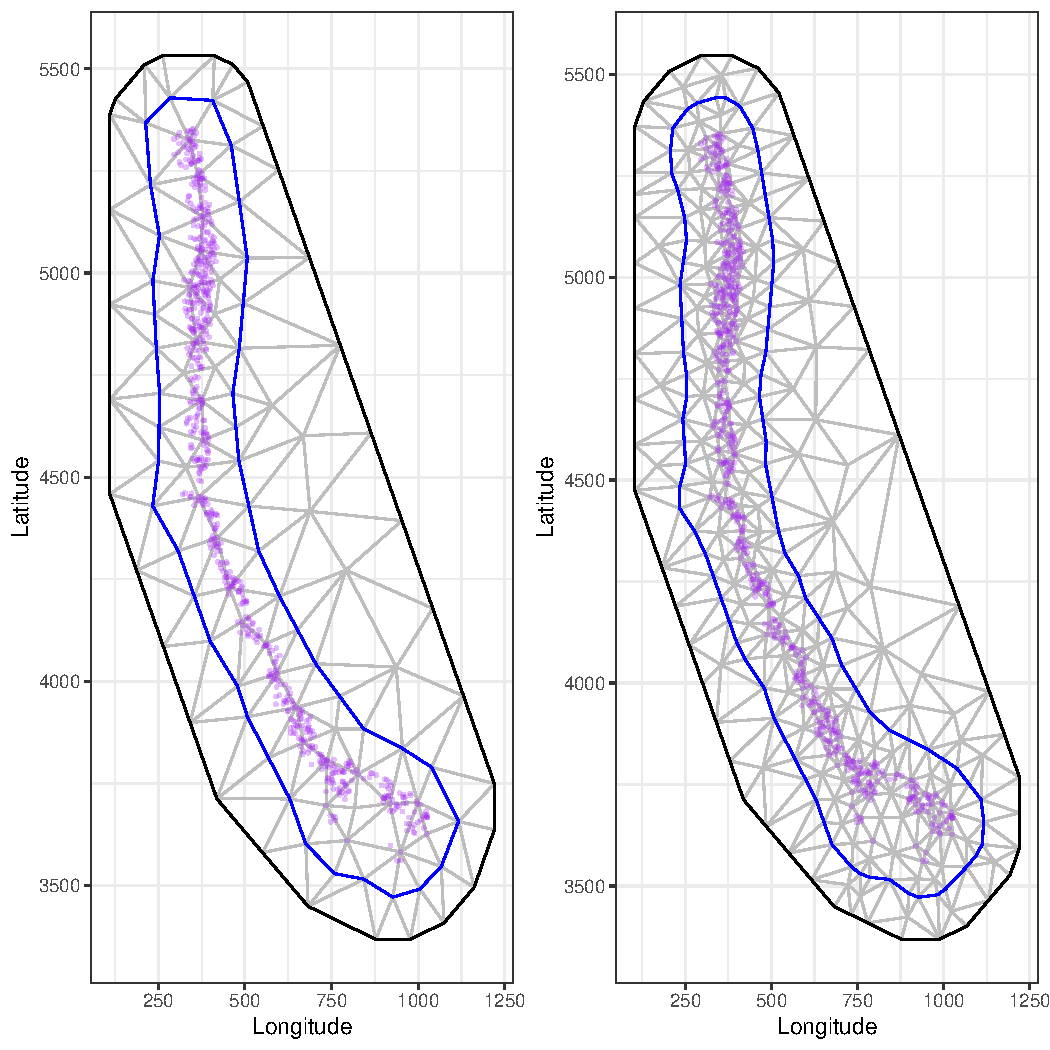
\includegraphics[width=4in]{figures/Figure_01.pdf}
  \caption{Example of two meshes constructed for the California Current
  Ecosystem, using the 2018 WCGBTS survey data. Cutoff values of 80 and 20 km
are used, translating into 110 and 394 knots (vertices) respectively. The blue
polygon illustrates the boundary between the inner and outer mesh where the
outer mesh has a larger maximum triangle edge length.}
  \label{fig:meshes}
\end{figure}

\break

\begin{figure}[htb]
  \centering
  \includegraphics[width=5in]{figures/Figure_02.pdf}
  \caption{(a) Sampled ocean temperature from the 2018 WCGBTS survey. Sample
  locations further offshore are typically colder and at greater depth. (b--c)
Average point-wise log-likelihood as a function of mesh features (b) cutoff
distance and (c) number of vertices, where the log-likelihood is calculated for
training and test datasets and normalized by the number of samples in each
using 10-fold cross validation with random fold assignments.}
  \label{fig:temperature}
\end{figure}

\break

\begin{figure}[htb]
  \centering
  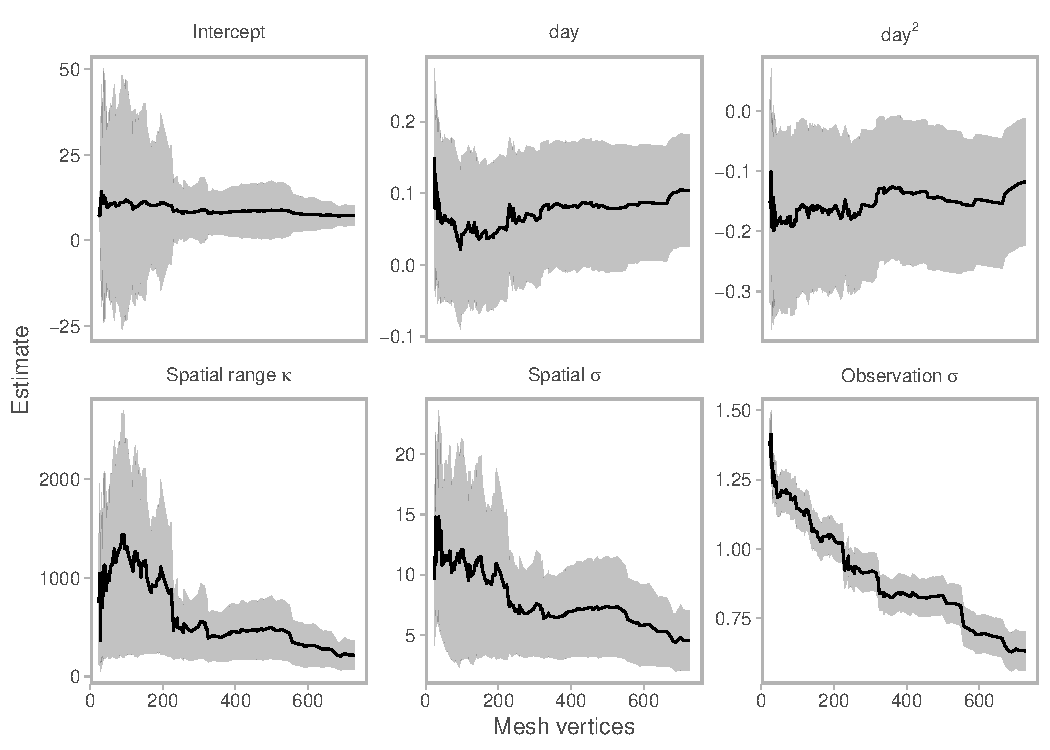
\includegraphics[width=5in]{figures/Figure_02b.pdf}
  \caption{Estimated fixed effect parameters (top row) and spatial parameters
  (bottom row) as a function of mesh vertices (more vertices translates to a
smaller cutoff distance in creating the mesh). The panels `day' and `day2'
represent the linear and quadratic effects of day of year. Solid lines
represent mean estimates, and shaded ribbons represent 95\% confidence
intervals.}
  \label{fig:temperaturepars}
\end{figure}

\break

\begin{figure}[htb]
  \centering
  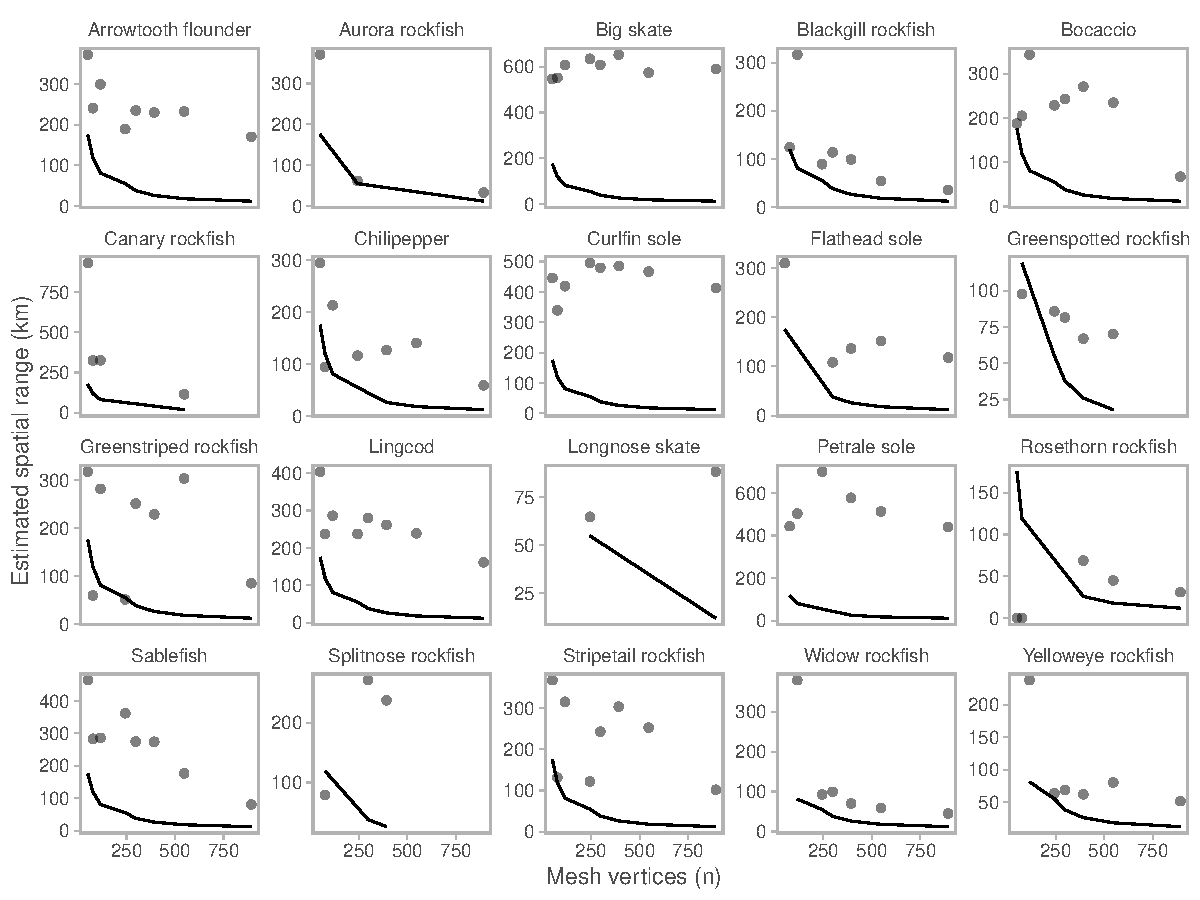
\includegraphics[width=\textwidth]{figures/groundfish_range_v_n.pdf}
  \caption{Estimated spatial range as a function of mesh vertices, for 20
  groundfish species included in our occurrence modeling (the mesh cutoff
distance corresponding to each vertex is shown as a solid black line). Colored
points represent different strip widths used for latitudinal spatial block
cross validation, and dark grey points represent results from cross validation
with random fold assignment.}
  \label{fig:gfrange}
\end{figure}

\break

\begin{figure}[htb]
  \centering
  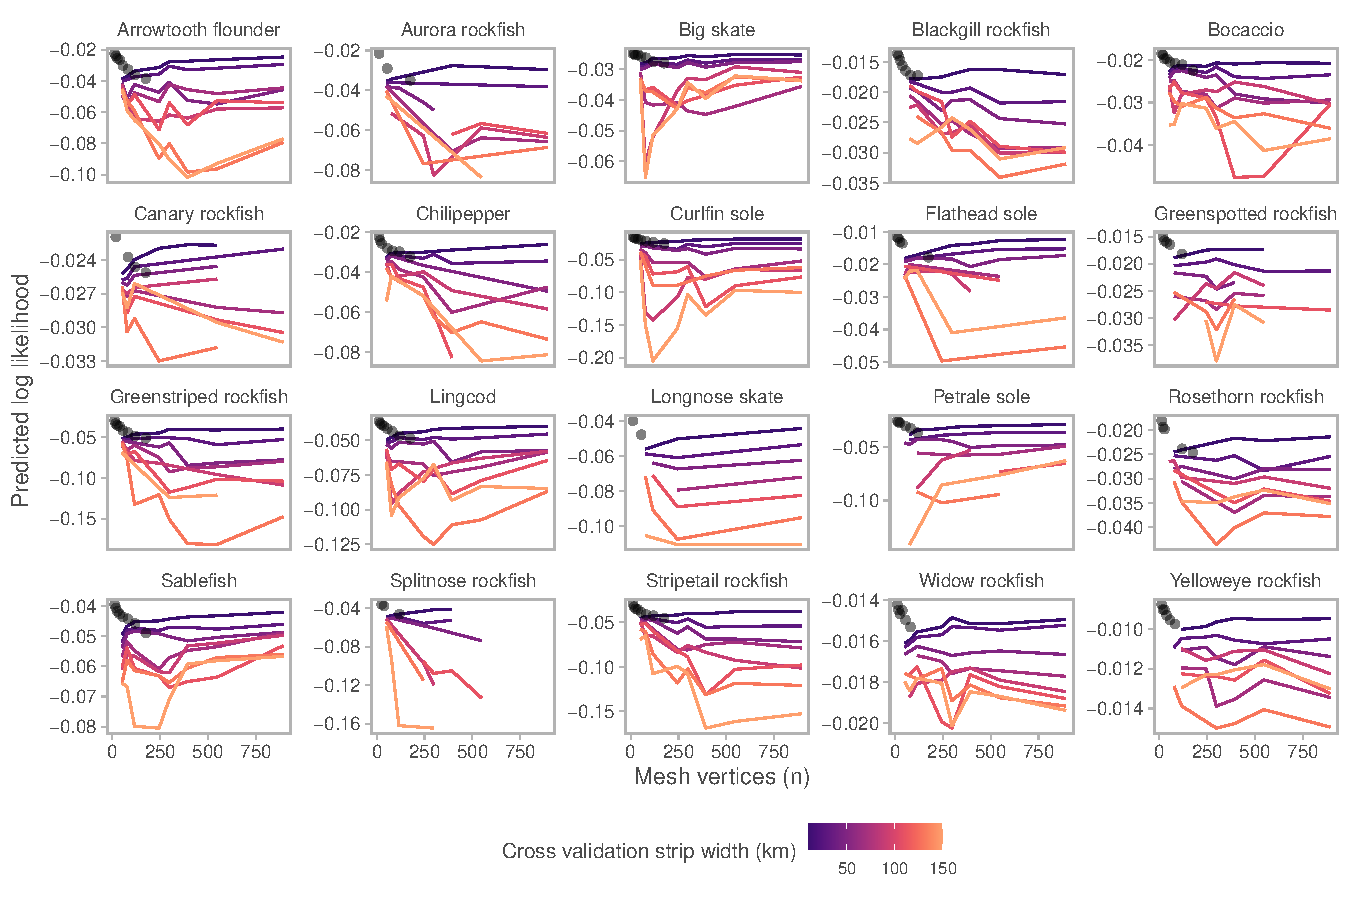
\includegraphics[width=\textwidth]{figures/groundfish_loglik_v_vertices.pdf}
  \caption{Estimated predictive log-likelihood as a function of mesh vertices
  (more vertices translates to a smaller cutoff distance in creating the mesh),
for 20 groundfish species included in our occurrence modeling. Colored points
represent different strip widths used for latitudinal spatial block cross
validation, and dark grey points represent results from cross validation with
random fold assignment.}
  \label{fig:gfloglik}
\end{figure}

\break

\begin{figure}[htb]
  \centering
  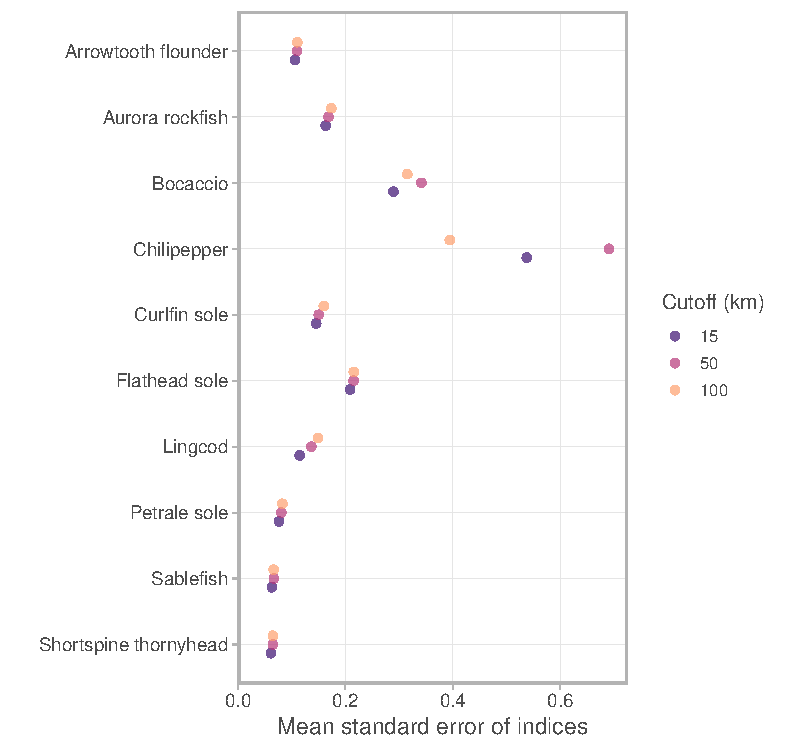
\includegraphics[width=4in]{figures/mean_index_se.pdf}
  \caption{Mean standard errors of biomass estimates (log space) estimated for
  each species across three mesh resolutions (larger cutoff distances result in
coarser meshes).}
  \label{fig:gfse}
\end{figure}

\bibliography{how-many-knots}

\renewcommand{\thefigure}{S\arabic{figure}}
\renewcommand{\thetable}{S\arabic{table}}
\setcounter{figure}{0}
\setcounter{table}{0}
\setcounter{section}{0}
\setcounter{subsection}{0}
\setcounter{subsubsection}{0}
\resetlinenumber
\setcounter{page}{1}
\setcounter{equation}{0}


\begin{figure}[htb]
  \centering
  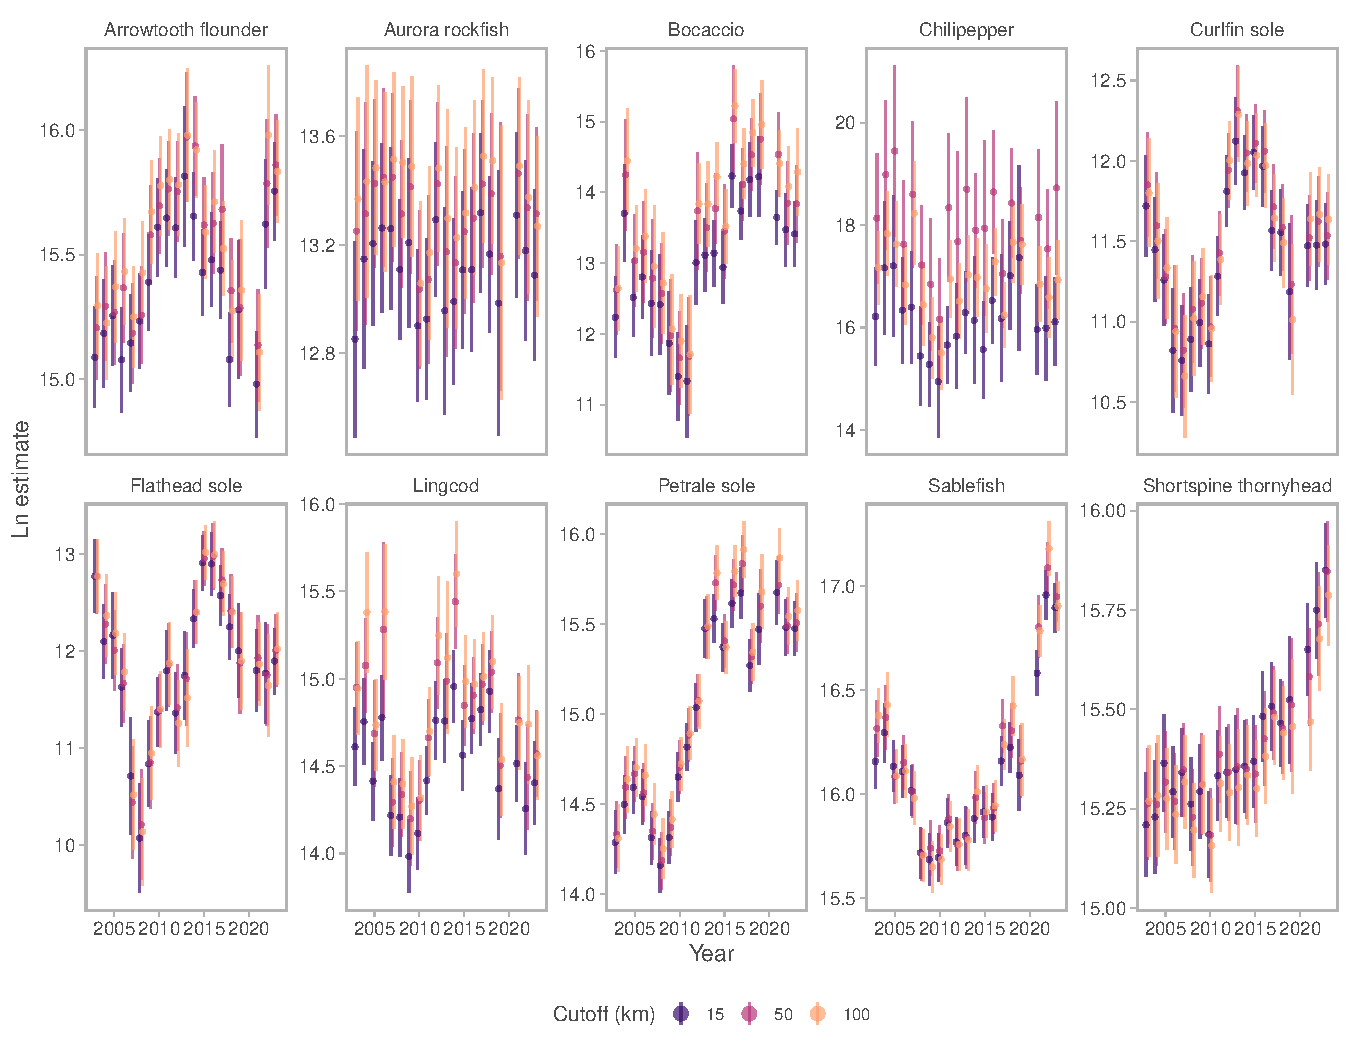
\includegraphics[width=\textwidth]{figures/SI_figure_indices.pdf}
  \caption{Time series of biomass estimates estimated for each species, across
  three mesh resolutions (larger cutoff distances result in coarser meshes).}
  \label{fig:gfts}
\end{figure}

\break

\begin{figure}[htb]
  \centering
  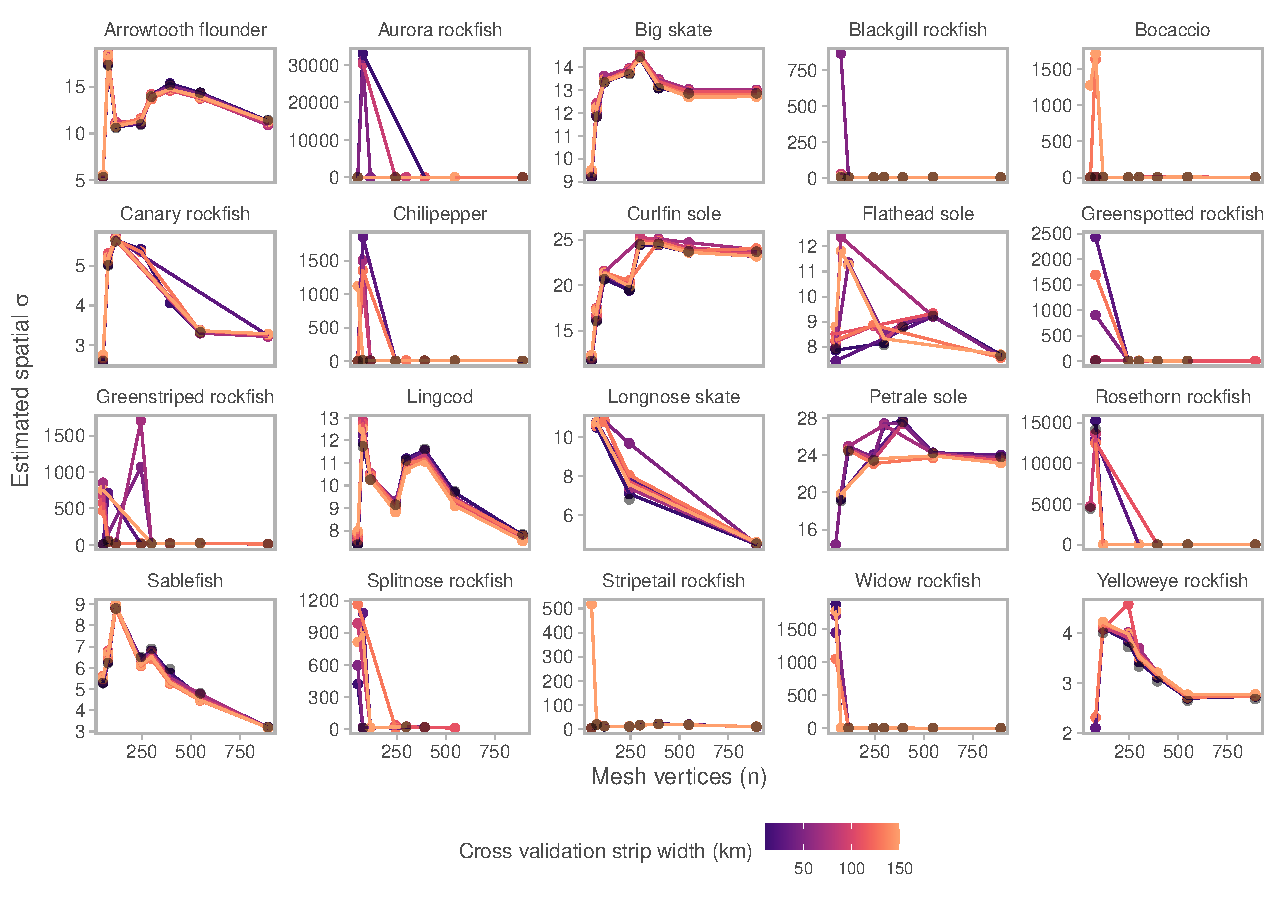
\includegraphics[width=\textwidth]{figures/groundfish_sigmaO_v_vertices.pdf}
  \caption{
Estimated spatial standard deviation as a function of mesh vertices (more
vertices translates to a smaller cutoff distance in creating the mesh), for 20
groundfish species included in our occurrence modeling. Colored points
represent different strip widths used for latitudinal spatial block cross
validation, and dark grey points represent results from cross validation with
random fold assignment.}
  \label{fig:gfsigmaO}
\end{figure}

\break

\begin{figure}[htb]
  \centering
  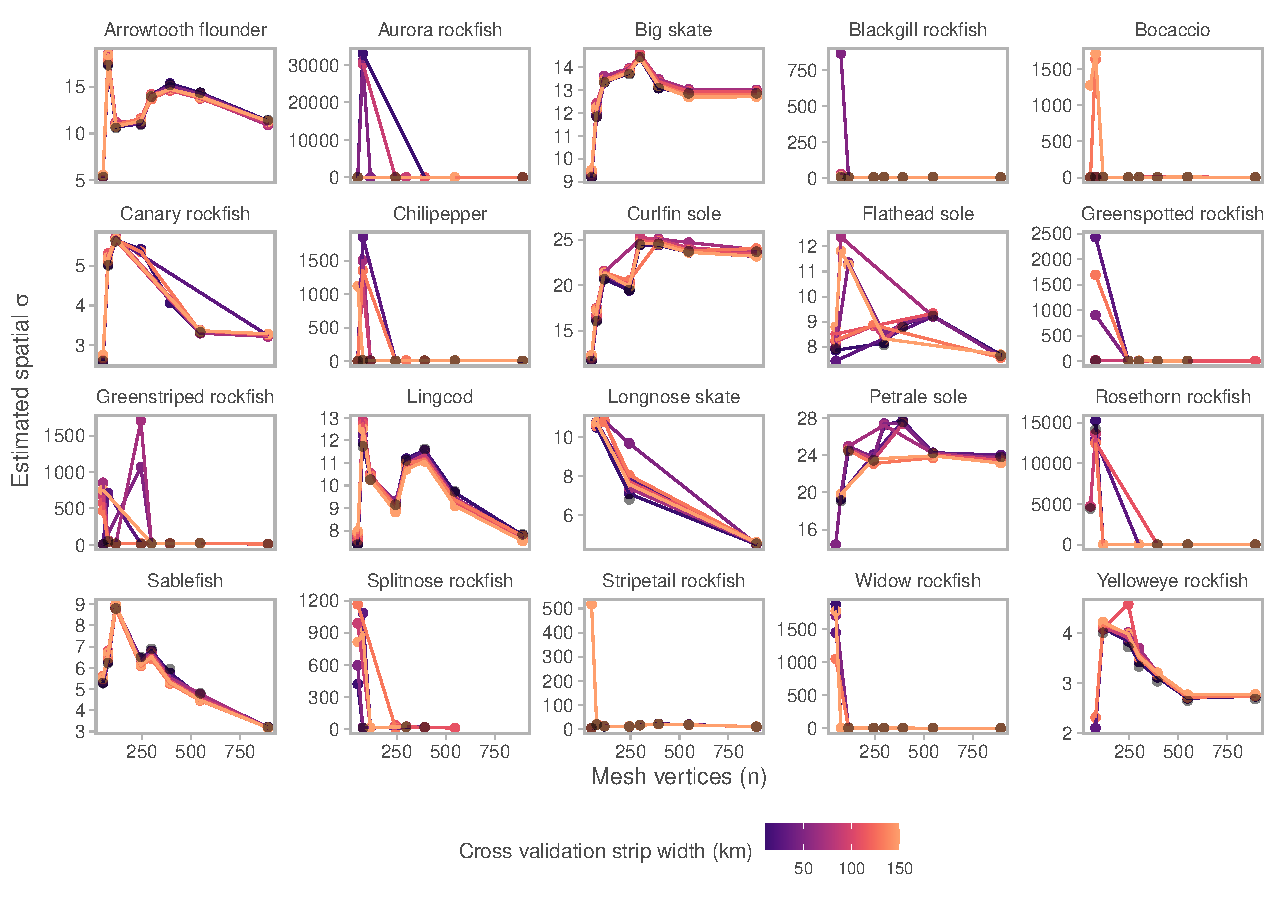
\includegraphics[width=\textwidth]{figures/groundfish_sigmaO_v_vertices.pdf}
  \caption{
Estimated spatiotemporal standard deviation as a function of mesh vertices
(more vertices translates to a smaller cutoff distance in creating the mesh),
for 20 groundfish species included in our occurrence modeling. Colored points
represent different strip widths used for latitudinal spatial block cross
validation, and dark grey points represent results from cross validation with
random fold assignment.}
\label{fig:gfsigmaE}
\end{figure}

\break

\begin{figure}[htb]
  \centering
  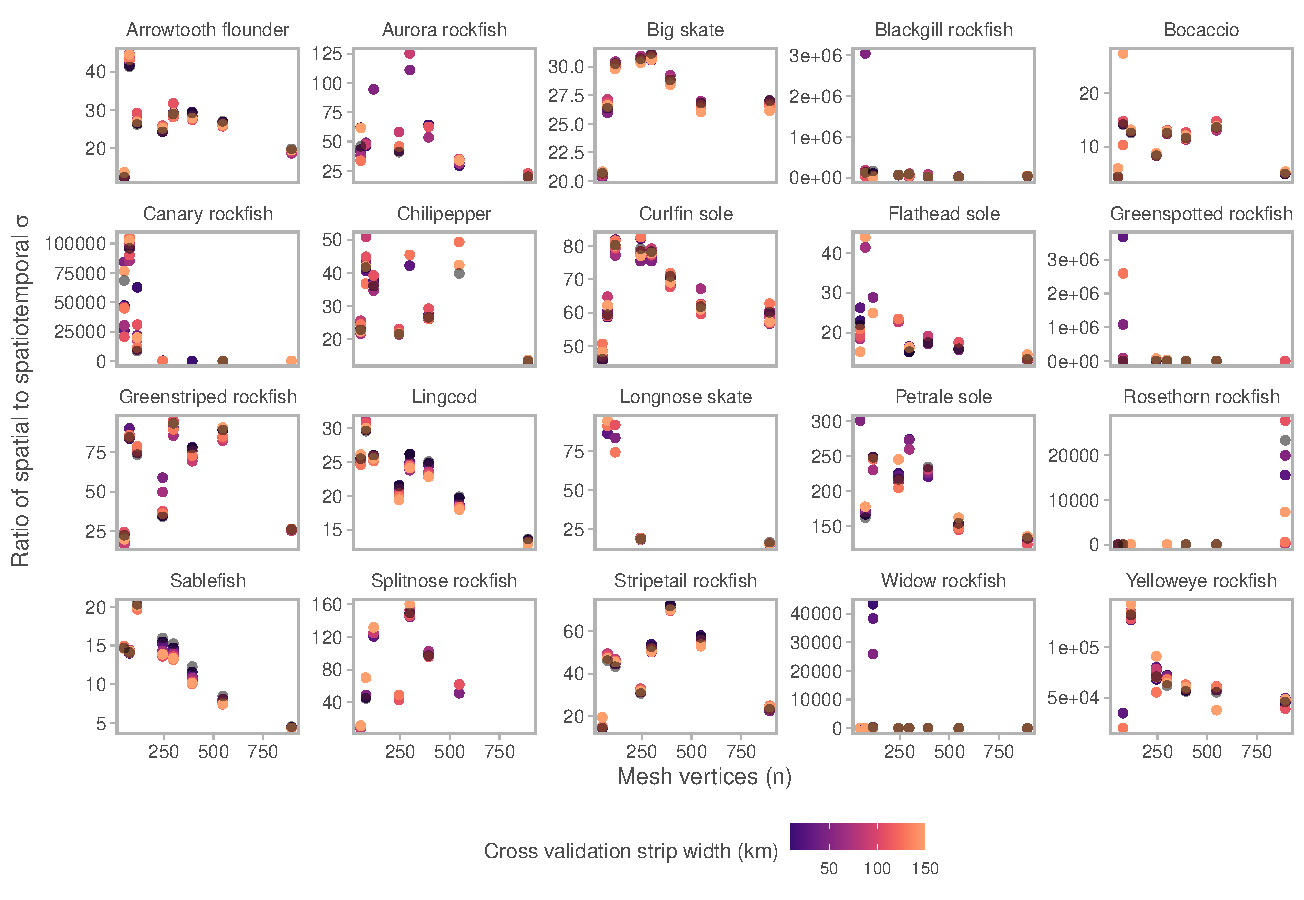
\includegraphics[width=\textwidth]{figures/groundfish_sigmaRatio_v_vertices.pdf}
  \caption{
  Ratio of estimated spatial standard deviation to estimated spatiotemporal
standard deviation as a function of mesh vertices (more vertices translates to
a smaller cutoff distance in creating the mesh), for 20 groundfish species
included in our occurrence modeling. Colored points represent different strip
widths used for latitudinal spatial block cross validation, and dark grey
points represent results from cross validation with random fold assignment.}
\label{fig:gfsigmaRatio}
\end{figure}

% species <- read.csv(here::here("species_names.csv"))
% species$sci_name <- paste0("\\textit{", species$sci_name, "}")
% knitr::kable(species, caption = "Table of groundfish species included in our encounter probability modeling.", col.names = c("Common name", "Scientific name", "Proportion of positive tows"), format = "latex", booktabs = TRUE, escape = FALSE, linesep = "")
%

\begin{table}
\caption{\label{tab:gf} Table of groundfish species included in our encounter probability modeling.}
\centering
\begin{tabular}[t]{llr}
\toprule
Common name & Scientific name & Proportion of positive tows\\
\midrule
Arrowtooth flounder & \textit{Atheresthes stomias} & 0.36\\
Aurora rockfish & \textit{Sebastes aurora} & 0.13\\
Big skate & \textit{Raja binoculata} & 0.16\\
Blackgill rockfish & \textit{Sebastes melanostomus} & 0.06\\
Bocaccio & \textit{Sebastes paucispinis} & 0.08\\
Canary rockfish & \textit{Sebastes pinniger} & 0.08\\
Chilipepper rockfish & \textit{Sebastes goodei} & 0.15\\
Curlfin sole & \textit{Pleuronichthys decurrens} & 0.12\\
Darkblotched rockfish & \textit{Sebastes crameri} & 0.18\\
Flathead sole & \textit{Hippoglossoides elassodon} & 0.08\\
Greenspotted rockfish & \textit{Sebastes chlorostictus} & 0.06\\
Greenstriped rockfish & \textit{Sebastes elongatus} & 0.26\\
Lingcod & \textit{Ophiodon elongatus} & 0.33\\
Longnose skate & \textit{Raja rhina} & 0.60\\
Longspine thornyhead & \textit{Sebastolobus altivelis} & 0.35\\
Petrale sole & \textit{Eopsetta jordani} & 0.43\\
Redbanded rockfish & \textit{Sebastes babcocki} & 0.08\\
Rex sole & \textit{Glyptocephalus zachirus} & 0.62\\
Rosethorn rockfish & \textit{Sebastes helvomaculatus} & 0.08\\
Sablefish & \textit{Anoplopoma fimbria} & 0.67\\
Sharpchin rockfish & \textit{Sebastes zacentrus} & 0.07\\
Shortspine thornyhead & \textit{Sebastolobus alascanus} & 0.51\\
Splitnose rockfish & \textit{Sebastes diploproa} & 0.20\\
Stripetail rockfish & \textit{Sebastes saxicola} & 0.22\\
Widow rockfish & \textit{Sebastes entomelas} & 0.04\\
Yelloweye rockfish & \textit{Sebastes ruberrimus} & 0.02\\
Yellowtail rockfish & \textit{Sebastes flavidus} & 0.07\\
\bottomrule
\end{tabular}
\end{table}

\break

\end{document}

